\chapter{Σχεδιασμός}
\InitialCharacter{Σ}το κεφάλαιο περιγράφονται αναλυτικά τα αντικείμενα που σχεδιάστηκαν στο πλαίσιο της εργασίας.

Αρχικά,
ορίστηκε μία δηλωτική γλώσσα ορισμού μοντέλων διεπαφών \en{(Domain-Specific Language - DSL)}.
Χρησιμοποιώντας τη μπορεί κανείς να περιγράψει μία προγραμματιστική διεπαφή τύπου \en{REST},
προσδιορίζοντας όλα τα χαρακτηριστικά της.

Στη συνέχεια, τα χαρακτηριστικά αυτά μοντελοποιήθηκαν με τρόπο αντικειμενοστρεφή, δηλαδή ως ξεχωριστές οντότητες.
Με άλλα λόγια, θεωρούμε πως μία προγραμματιστική διεπαφή είναι ένα σύνολο αντικειμένων,
το καθένα με τις δικές του ξεχωριστές ιδιότητες και λειτουργίες,
που αλληλεπιδρούν μεταξύ τους. 

Για να επιβεβαιώσουμε την ορθή λειτουργία της εργασίας,
σχεδιάστηκαν σενάρια ελέγχου για καθένα από τα αντικείμενα που αναπαριστούν τόσο την προγραμματιστική διεπαφή, 
όσο και τα χαρακτηριστικά της. 
Αυτά τα σενάρια ελέγχου επιβεβαιώνουν όχι μόνο ότι η διεπαφή που αναπαριστάται αντιστοιχεί στις προδιαγραφές που δίνει ο χρήστης,
αλλά ακόμα και ότι δεν θα δημιουργηθεί μία διεπαφή με προφανή προβλήματα,
όπως για παράδειγμα διεπαφή χωρίς τελικά σημεία ή μέθοδος χωρίς αίτηση.

Τέλος, για την ολοκληρωμένη λειτουργία του συστήματος,
σχεδιάστηκε μία γεννήτρια κώδικα.
Αυτή είναι ένα πρόγραμμα που δέχεται την αναπαράσταση μιας προγραμματιστικής διεπαφής
και παράγει σενάρια ελέγχου και βοηθητικά εργαλεία.
Για να το καταφέρει αυτό, 
αξιοποιεί τα πρότυπα που της παρέχονται,
δηλαδή έτοιμα κομμάτια κώδικα 
που προσαρμόζονται με βάση τα δεδομένα εισόδου. 

\begin{figure}
    \centering
	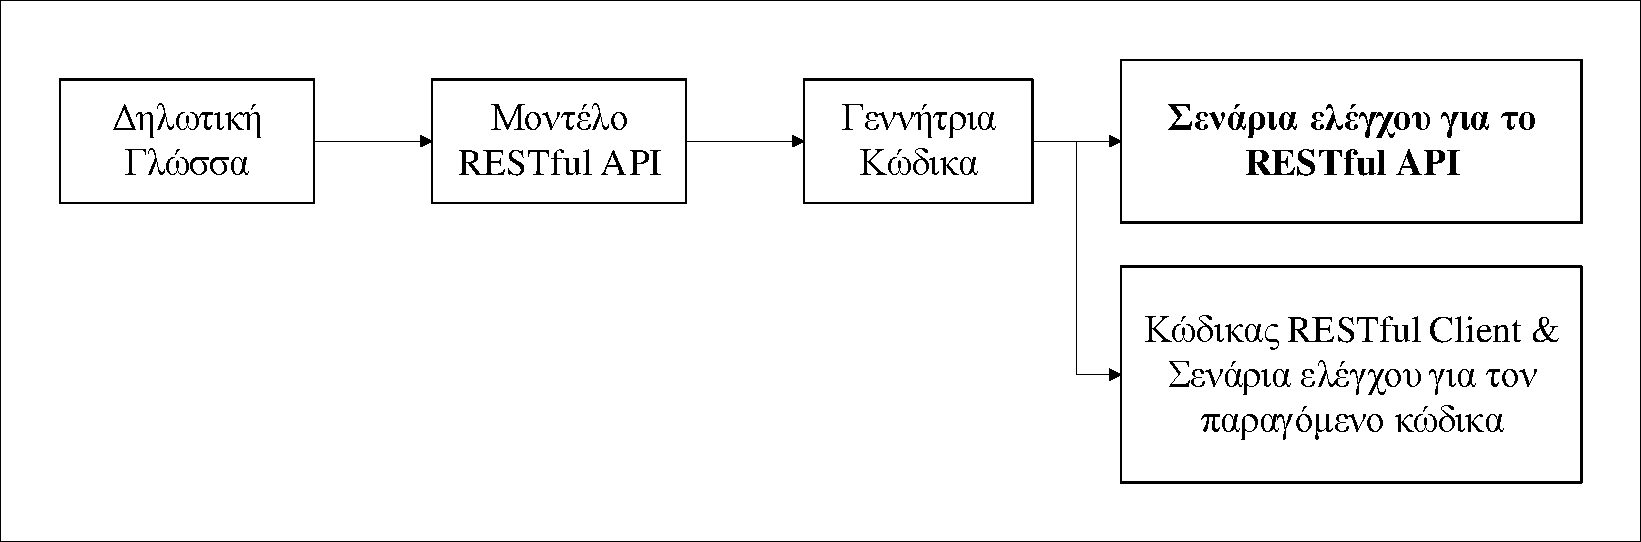
\includegraphics[width=\textwidth]{figures/DSL.pdf} 
    \caption{Διάγραμμα ροής χρήσης εργασίας}
    \label{figure3.1}
\end{figure} 

\section{Δηλωτική γλώσσα ορισμού μοντέλων διεπαφών}

Βασικός σκοπός της εργασίας είναι να μπορεί οποιοσδήποτε προγραμματιστής να περιγράφει με απλό τρόπο
τα χαρακτηριστικά μιας προγραμματιστικής διεπαφής τύπου \en{REST}
και να παίρνει ένα σύνολο από σενάρια ελέγχου που την καλύπτουν κατά το δυνατό περισσότερο.
Για τον λόγο αυτό ορίστηκε μία δηλωτική γλώσσα ορισμού μοντέλων διεπαφών.
Μέσω αυτής, μπορεί κανείς να προσδιορίσει με σαφήνεια όλες τις παραμέτρους που υποστηρίζονται,
δίχως να απαιτείται να έχει γνώση του εσωτερικού τρόπου λειτουργίας της εργασίας
και πώς αυτή μοντελοποιεί τα δεδομένα.

Για παράδειγμα,
ας υποθέσουμε πως έχουμε μία προγραμματιστική διεπαφή τύπου \en{REST}
με διεύθυνση βάσης '\emph{\en{/observatory/api}}' και ετικέτα '\emph{\en{my test api}}'.
Έστω ότι αυτή η διεπαφή διαθέτει ένα τελικό σημείο διαπίστευσης χρηστών,
το οποίο υποστηρίζει μέσω της μεθόδου \en{POST} δύο παραμέτρους σώματος για όνομα χρήστη και κωδικό πρόσβασης
και σε περίπτωση επιτυχίας επιστρέφει απάντηση με κωδικό κατάστασης 201.

Ο τρόπος με τον οποίο εκφράζονται τα παραπάνω στοιχεία μέσω της δηλωτικής γλώσσας είναι ο ακόλουθος:

\selectlanguage{english}
\begin{lstlisting}
api {
\end{lstlisting}
\begin{lstlisting}[deletekeywords={api}]
    baseUrl '/test/api'
    label   'my test api'
    endpoint(/login) {
        label 'Endpoint login'
        description 'Endpoint for user login with username and password'
        method(POST) {
            request(URL) {
                withBodyParameter(username, String)
                withBodyParameter(password, String)
            }
            response(JSON) {
                withStatus(201) {
                    body 'Created'
                }
            }
        }
    }
}
\end{lstlisting}
\selectlanguage{greek}

Η δηλωτική γλώσσα ορισμού μοντέλων διεπαφών σχεδιάστηκε με γνώμονα την ακριβέστερη απεικόνιση των χαρακτηριστικών ενός \en{RESTful API}.
Κοιτώντας μία προγραμματιστική διεπαφή εκφρασμένη στη συγκεκριμένη γλώσσα 
μπορεί κανείς εύκολα να κατανοήσει τις λειτουργίες και τις δυνατότητές της.
Παράλληλα κάθε έκφραση της γλώσσας είναι ξεκάθαρη 
και δεν αφήνει αμφιβολίες στον προγραμματιστή ως προς τη χρήση της.

Στο τέλος του κεφαλαίου παρατίθεται η πλήρης γραμματική της γλώσσας.

\section{Μοντελοποίηση προγραμματιστικής διεπαφής τύπου \en{REST}}
Θεωρούμε ότι κάθε προγραμματιστική διεπαφή (\en{API}) περιλαμβάνει τουλάχιστον ένα τελικό σημείο (\en{endpoint}), 
που το καθένα έχει τις δικές του μεθόδους (\en{methods}).
Κάθε μέθοδος έχει από μία αίτηση (\en{request}) και μία απάντηση (\en{response}).
Μία αίτηση αποτελείται από κεφαλίδες (\en{headers}) και παραμέτρους (\en{parameters}), 
οι οποίες μπορεί να είναι είτε σώματος (\en{body}) είτε αιτήματος (\en{query}).
Από την άλλη,
μία απάντηση αποτελείται από κεφαλίδες και μία κατάσταση (\en{status}).

\begin{figure}[!b]
    \centering
	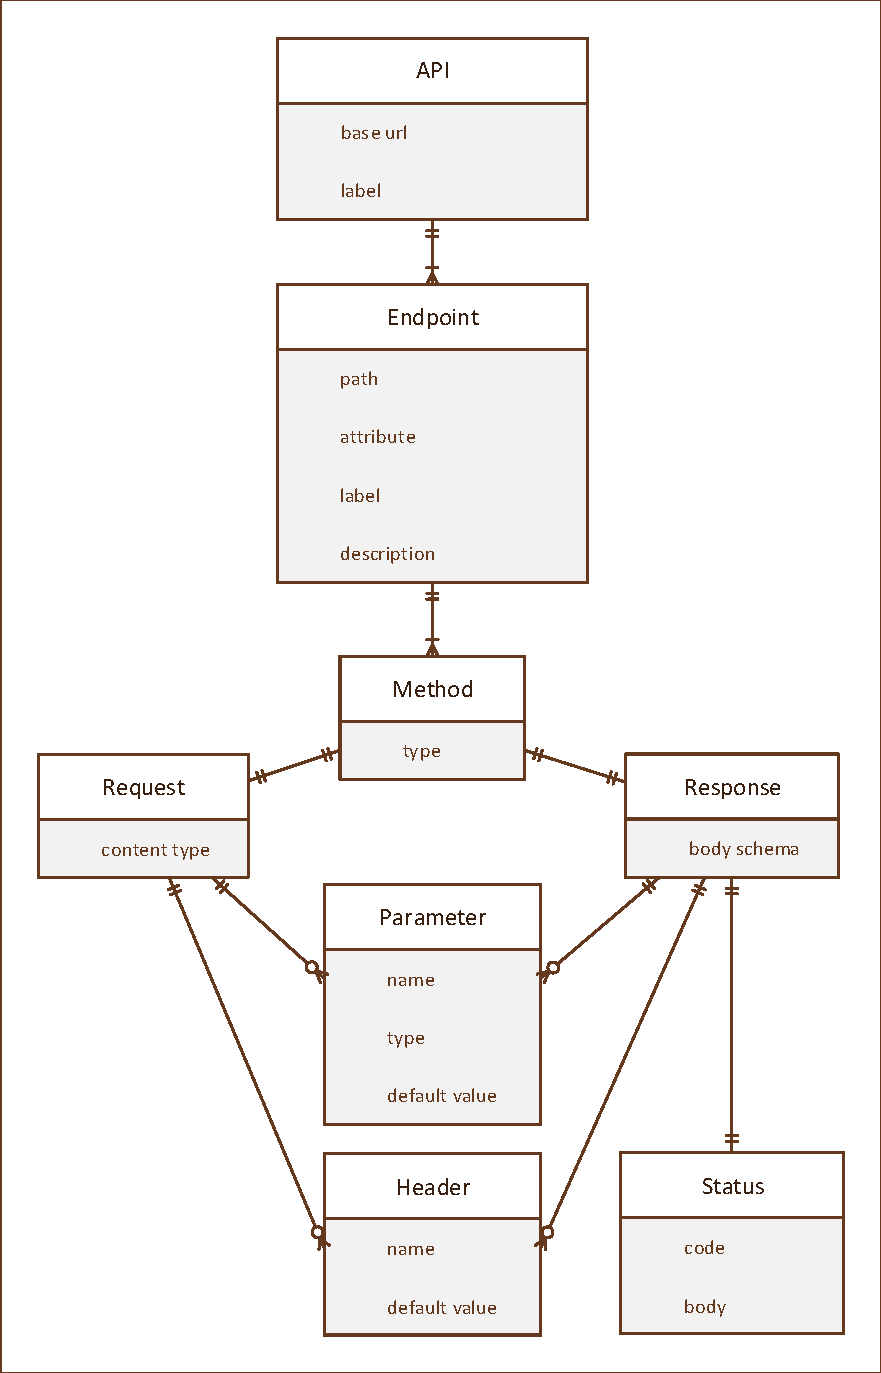
\includegraphics[height=18cm,keepaspectratio]{figures/ERD_eng.pdf} 
    \caption{Διάγραμμα οντοτήτων-συσχετίσεων}
    \label{figure3.2}
\end{figure} 

\begin{itemize}
    \item \underline{Προγραμματιστική Διεπαφή τύπου \en{REST} (\en{RESTful API})}
    
    Μία προγραμματιστική διεπαφή τύπου \en{REST},
    όπως περιγράφηκε και στο Κεφάλαιο 2,
    είναι ένα τμήμα λογισμικού ενός συστήματος
    που παρέχει σε προγραμματιστές πρόσβαση σε ένα σύνολο από λειτουργίες και διαδικασίες
    και ακολουθεί το αρχιτεκτονικό στυλ \en{REST (Representational State Transfer)}.

    Περιλαμβάνει:
    \begin{itemize}
        \item Μία διεύθυνση βάσης (\en{base URL}), όπως \en{https://api.example.com/}
        \item Μία ετικέτα (προαιρετικό), όπως '\en{API example}'
        \item Ένα τουλάχιστον τελικό σημείο (\en{endpoint})
    \end{itemize}

    
\item \underline{Τελικό Σημείο (\en{Endpoint})}

Ένα τελικό σημείο είναι ο δίαυλος επικοινωνίας μιας προγραμματιστικής διεπαφής με τον Παγκόσμιο Ιστό.

Είναι μία πύλη που επιτρέπει σε προγραμματιστές να στείλουν συγκεκριμένα αιτήματα προς τη διεπαφή και να τους επιστραφούν απαντήσεις.
Στην πράξη κάθε τελικό σημείο αναπαριστά μία ομάδα παρεμφερών λειτουργιών που υποστηρίζει η διεπαφή,
όπως αλληλεπίδραση με δεδομένα ή εκτέλεση εντολών.

Συνήθως ένα τελικό σημείο έχει το δικό του μονοπάτι που λειτουργεί ως πρόθεμα στη διεύθυνση της διεπαφής.

Περιλαμβάνει:
\begin{itemize}
    \item Ένα μονοπάτι
    \item Μία ετικέτα (προαιρετικό)
    \item Μία περιγραφή (προαιρετικό)
    \item Ένα ή περισσότερα προσδιοριστικά (προαιρετικά)
    \item Μία τουλάχιστον μέθοδο
\end{itemize}

\item \underline{Μέθοδος (\en{Method})}

Μία μέθοδος είναι μια επιθυμητή εντολή σε κάποιον πόρο του συστήματος.
Οι δυνατές εντολές είναι ορισμένες από το Πρωτόκολλο Μεταφοράς Υπερκειμένου (\en{HyperText Transfer Protocol, HTTP}) 
και δρουν σε ένα συγκεκριμένο τελικό σημείο της διεπαφής \cite{fielding1999hypertext}.
Σε αυτό μεταφέρουν ένα αίτημα και από αυτό δέχονται μία απάντηση.

Περιλαμβάνει:
\begin{itemize}
    \item Έναν τύπο
    \item Μία αίτηση
    \item Μία απάντηση
\end{itemize}

Στο πλαίσιο της εργασίας θεωρούμε ως επιτρεπτές τιμές του τύπου μιας μεθόδου τις \en{GET, POST, PUT, PATCH} και \en{DELETE}.

\item \underline{Αίτηση (\en{Request})}

Μία αίτηση είναι ένα μήνυμα που στέλνει ένας χρήστης ή ένα πρόγραμμα σε μια διεπαφή.
Αυτό το μήνυμα περιέχει όλες τις απαραίτητες πληροφορίες που χρειάζεται ο διακομιστής που θα την λάβει για να την διεκπεραιώσει.
Κάθε αίτηση πραγματοποιείται σε μια συγκεκριμένη διεύθυνση που συνήθως είναι ένα τελικό σημείο μιας διεπαφής.

Περιλαμβάνει:
\begin{itemize}
    \item Έναν τύπο περιεχομένου (\en{MIME})
    \item Ένα σύνολο από κεφαλίδες (προαιρετικό)
    \item Ένα σύνολο από παραμέτρους σώματος (προαιρετικό)
    \item Ένα σύνολο από παραμέτρους αιτήματος (προαιρετικό)
\end{itemize}

Ως τύπος περιεχομένου ορίζεται ένα αναγνωριστικό της μορφής 'τύπος/υπότυπος'
που περιγράφει τη μορφή του περιεχομένου της αίτησης.

Για τους σκοπούς της διπλωματικής,
οι τύποι περιεχομένου που υποστηρίζονται είναι αποκλειστικά οι '\en{application/json}' και '\en{application/x-www-form-urlencoded}'.

\item \underline{Απάντηση (\en{Response})}

Μία απάντηση είναι το αποτέλεσμα που παράγεται από μια διεπαφή που δέχεται μία αίτηση.
Δίνεται από το σύστημα που έχει την διεπαφή στον χρήστη ή το πρόγραμμα που στέλνει την αίτηση στο ίδιο τελικό σημείο που στάλθηκε αυτή.

Περιλαμβάνει:
\begin{itemize}
    \item Ένα σχήμα σώματος
    \item Ένα σύνολο από κεφαλίδες (προαιρετικό)
    \item Μία κατάσταση
\end{itemize}

Στο πλαίσιο της διπλωματική εργασίας
επιλέχθηκε η αναφορά του σχήματος του σώματος της απάντησης ως προαπαιτούμενο για την αυτόματη παραγωγή των αντιστοίχων σεναρίων ελέγχου.

Για την ακρίβεια, υποστηρίζονται οι μορφές \en{JSON}, συμβολοσειράς και ακεραίου αριθμού. 

\item \underline{Κεφαλίδα (\en{Header})}

Μία κεφαλίδα είναι το μέρος ενός μηνύματος αίτησης ή απάντησης 
που περιλαμβάνει πρόσθετες πληροφορίες επικοινωνίας.

Περιλαμβάνει:
\begin{itemize}
    \item Ένα όνομα
    \item Μία προεπιλεγμένη τιμή σε περίπτωση που είναι προαιρετική και δεν παρέχεται
\end{itemize}

Μία Κεφαλίδα πρέπει επίσης να δηλώνεται αν είναι υποχρεωτική ή προαιρετική.

\item \underline{Παράμετρος (\en{Parameter})}

Μία παράμετρος είναι ένα στοιχείο ενός μηνύματος
που βοηθάει στον προσδιορισμό παραμέτρων και στην μεταφορά πρόσθετων πληροφοριών.

Μπορεί να είναι είναι στο σώμα του μηνύματος, είτε στη διεύθυνση αιτήματος.

Περιλαμβάνει:
\begin{itemize}
    \item Ένα όνομα
    \item Έναν τύπο
    \item Μία προεπιλεγμένη τιμή σε περίπτωση που είναι προαιρετική και δεν παρέχεται
\end{itemize}

Μία παράμετρος πρέπει επίσης να δηλώνεται αν είναι υποχρεωτική ή προαιρετική.

\item \underline{Κατάσταση (\en{Status})}

Μία κατάσταση είναι το τμήμα της απάντησης που εκδίδεται από τον διακομιστή
και περιγράφει συνοπτικά το αποτέλεσμα της αίτησης.

Περιλαμβάνει:
\begin{itemize}
    \item Έναν κωδικό (πχ. 201)
    \item Ένα σώμα (πχ. '\en{Created}')
\end{itemize}

Ανάλογα με το είδος του αποτελέσματος της αίτησης,
έχουν καθιερωθεί οι ακόλουθες ομάδες κωδικών κατάστασης:

\begin{itemize}
    \item Ενημερωτικές απαντήσεις (100–199)
    \item Επιτυχείς απαντήσεις (200–299)
    \item Ανακατευθύνσεις (300–399)
    \item Προβλήματα χρήστη (400–499)
    \item Προβλήματα διακομιστή (500–599)
\end{itemize}

\end{itemize}

\section{Σενάρια ελέγχου της μοντελοποίησης}
Για να είμαστε βέβαιοι πως η υλοποίηση των παραπάνω αντικειμένων δεν έχει λάθη,
σχεδιάστηκαν σενάρια ελέγχου για καθένα από αυτά.
Έτσι, για κάθε αντικείμενο ελέγχουμε αν τα δεδομένα που του δίνουμε κατά τη δημιουργία 
είναι ίδια με αυτά που επιστρέφονται από αυτό που έχει παραχθεί.

Επιπλέον ελέγχουμε αν έχουν δοθεί τα υποχρεωτικά χαρακτηριστικά,
τα οποία ανάλογα την προδιαγραφή είναι:

\begin{itemize}
    \item Για την διεπαφή απαιτείται τουλάχιστον ένα τελικό σημείο.
    \item Για το τελικό σημείο απαιτείται το μονοπάτι και τουλάχιστον μία υποστηριζόμενη μέθοδος.
    \item Για τη μέθοδο απαιτούνται ο τύπος της, η αίτηση και η απάντηση.
    \item Για την απάντηση απαιτείται η κατάστασή της.
    \item Για την κεφαλίδα απαιτείται το όνομά της, ενώ σε περίπτωση που είναι υποχρεωτική απαιτείται και ένα προκαθορισμένο σώμα.
    \item Για την παράμετρο απαιτούνται το όνομά της και ο τύπος της, ενώ σε περίπτωση που είναι υποχρεωτική απαιτείται και ένα προκαθορισμένο σώμα.
    \item Τέλος, για την κατάσταση απαιτούνται ο κωδικός και το σώμα της.
\end{itemize}

Υπάρχουν ορισμένοι επιπρόσθετοι έλεγχοι για την ορθότητα των δεδομένων.
Έτσι, σε μία προγραμματιστική διεπαφή ελέγχουμε αν η διεύθυνση βάσης είναι έγκυρη διεύθυνση του Παγκοσμίου Ιστού
και σε μία κατάσταση αν ο κωδικός είναι εντός των υποστηριζόμενων ορίων (100-599).

\section{Γεννήτρια Κώδικα}
Έχοντας ορίσει αναλυτικά τις προδιαγραφές μιας διεπαφής προγραμματισμού τύπου \en{REST},
σχεδιάστηκε μία γεννήτρια κώδικα που λειτουργεί ως επεξεργαστής προτύπων.
Ένας επεξεργαστής προτύπων είναι ένα λογισμικό που συνδυάζει πρότυπα και μοντέλα δεδομένων 
με σκοπό την παραγωγή ενός τελικού κειμένου \cite{niemeyer2005learning}.

Η γεννήτρια κώδικα που σχεδιάστηκε χρησιμοποιεί ως μοντέλο δεδομένων την αναπαράσταση μιας διεπαφής
με τα χαρακτηριστικά που ορίστηκαν παραπάνω. 

Με τα πρότυπα που σχεδιάστηκαν,
η γεννήτρια κώδικα παράγει τα ακόλουθα:

\subsection{Πελάτης (\en{Client}) \en{RESTful API}}

Ο πελάτης διεπαφής είναι ένα λογισμικό που αξιοποιεί το πρωτόκολλο επικοινωνίας \en{HTTP}.
Με αυτό μπορούν να πραγματοποιηθούν όλες οι μορφές επικοινωνίας που δηλώνονται στις προδιαγραφές μιας διεπαφής.
Για τη διπλωματική εργασία είναι ένα απαραίτητο εργαλείο 
που στόχο έχει την εκτέλεση των τμημάτων των σεναρίων ελέγχου
που αφορούν την επικοινωνία με μία προγραμματιστική διεπαφή τύπου \en{REST}.

Για να το δημιουργήσει η γεννήτρια κώδικα,
αρχικά διαβάζει από τις προδιαγραφές της διεπαφής τη διεύθυνση βάσης,
καθώς και όλα τα τελικά σημεία που υποστηρίζονται.
Για καθένα από αυτά,
ελέγχει αν χρησιμοποιεί κάποιο προσδιοριστικό, 
καθώς και ποιες μεθόδους υποστηρίζει.
Λαμβάνεται υπόψη ακόμα και το σχήμα σώματος της απάντησης κάθε μεθόδου.  

\subsection{Σενάρια ελέγχου για τον παραγόμενο κώδικα με εικονικό διακομιστή (\en{Mock Server})}

Τα σενάρια ελέγχου με εικονικό διακομιστή είναι απαραίτητα για να βεβαιωθούμε πως ο πελάτης διεπαφής που θα δημιουργηθεί
θα εμφανίζει την επιθυμητή συμπεριφορά.

Η γεννήτρια κώδικα,
έχοντας παράξει τον πελάτη, 
χρησιμοποιεί τις προδιαγραφές της διεπαφής και
συντάσσει μια σειρά από σενάρια ελέγχου που περιλαμβάνουν την αποστολή και λήψη μηνυμάτων 
μέσα από τον πελάτη. 

Αρχικά αναλύει κάθε τελικό σημείο ως προς τις μεθόδους που υποστηρίζει,
ενώ παράλληλα ελέγχει αν χρησιμοποιεί κάποιο προσδιοριστικό.

Στη συνέχεια, προετοιμάζει μια εικονική αίτηση που θα χρησιμοποιηθεί για τους σκοπούς του ελέγχου.
Αυτή προκύπτει από τις προδιαγραφές της αίτησης κάθε μεθόδου και πιο συγκεκριμένα από τα παρακάτω στοιχεία:

Ανάλογα με τον τύπο περιεχομένου της αίτησης και πιο συγκεκριμένα αν αυτός είναι '\en{application/json}' ή '\en{application/x-www-form-urlencoded}',
παράγεται ένα αρχείο \en{JSON} ή μια συμβολοσειρά της μορφής '\en{field1=value1\&field2=value2}' με ζεύγη ονομάτων παραμέτρων και τιμών αντίστοιχα.
Σε κάθε περίπτωση περιλαμβάνονται τιμές για κάθε παράμετρο σώματος που υποστηρίζεται.

Με όμοιο τρόπο σχηματίζονται τιμές για κάθε κεφαλίδα και κάθε παράμετρο αίτησης σε μορφή πινάκων κατατεμαχισμού (\en{hashmap}).

Όπου χρειάζεται να μπει τιμή μεταβλητής σε παραμέτρους και κεφαλίδες,
έχουν επιλεγεί για τους σκοπούς της διπλωματικής εργασίας οι εξής τιμές:

\begin{itemize}
    \item Για συμβολοσειρές, τιμή της μορφής '\en{headerValue}'
    \item Για ακεραίους, ο αριθμός 42
    \item Για αριθμούς κινητής υποδιαστολής, ο αριθμός 42,5
    \item Για τύπους δεδομένων Αληθείας (\en{Boolean}), η τιμή Αληθής/\en{True}
\end{itemize}

Σε μεθόδους τύπου \en{GET, PUT, PATCH} και \en{DELETE} που χρησιμοποιούν προσδιοριστικό,
αυτό θεωρείται πως είναι ακέραιος αριθμός και για τους σκοπούς των ελέγχουν του ανατίθεται η τιμή 2.

Αμέσως μετά προδιαγράφεται ένας εικονικός διακομιστής (\en{Mock Server}).
Η λειτουργία του είναι όταν δέχεται στη διεύθυνση του τελικού σημείου
αίτηση με την αντίστοιχη μέθοδο και με τις κεφαλίδες και τις παραμέτρους σώματος και αίτησης των προδιαγραφών,
τότε να επιστρέφει μία συγκεκριμένη απάντηση στον πελάτη.
Αυτή θα έχει την κατάσταση,
τις κεφαλίδες της
και το σώμα της κατάστασης.
Το τελευταίο επιλέγεται ανάλογα με τον τύπο σχήματος και μπορεί να είναι είτε της μορφής \en{JSON},
είτε συμβολοσειρά είτε ακέραιος.

Η διαδικασία αυτή επαναλαμβάνεται για κάθε μέθοδο κάθε τελικού σημείου της διεπαφής.

\subsection{Σενάρια ελέγχου για το \en{RESTful API}}

Τέλος, τα σενάρια ελέγχου για το μοντέλο \en{RESTful API} παράγονται με παρόμοιο τρόπο με τα προαναφερθέντα,
με βασική διαφορά την έλλειψη εικονικού διακομιστή.
Αντί για αυτόν, η γεννήτρια κώδικα συντάσσει σενάρια ελέγχου που πραγματοποιούν αιτήσεις στη διεύθυνση και τη θύρα που έχουν οριστεί από τον χρήστη
και επαληθεύουν το αποτέλεσμα που δέχεται ο πελάτης διεπαφής.

Οι αιτήσεις προετοιμάζονται με τον ίδιο τρόπο ακριβώς με παραπάνω,
λαμβάνοντας υπόψη όλα τα χαρακτηριστικά της διεπαφής.

Οι έλεγχοι καλύπτουν:
\begin{itemize}
    \item Την ομαλή λειτουργία του διακομιστή και την επιτυχή σύνδεση σε αυτόν μέσω της θύρας που δίνεται.
    \item Τη δυνατότητα αποστολής μιας αίτησης με τις παραμέτρους και τις κεφαλίδες που υποστηρίζονται.
    \item Αν η απάντηση έχει τη μορφή που αναμένεται.
    \item Την ύπαρξη στις κεφαλίδες της απάντησης των πεδίων που αναμένονται.
    \item Την αποτυχία μιας αίτησης σε περίπτωση που λείπει μία υποχρεωτική παράμετρος ή κεφαλίδα.
\end{itemize}

\section{Γραμματική δηλωτικής γλώσσας ορισμού μοντέλων διεπαφών}

\selectlanguage{english}
\begin{lstlisting}
API                 : '{' 'baseUrl' BASEURL ('label' LABEL)? (('endpoint(' PATH+ ')' | ('endpoint(' PATH ',' ATTRIBUTE ')') ENDPOINT)+ '}'

ENDPOINT            : '{' ('label' LABEL)? ('description' DESCRIPTION)? 'method(' METHODTYPE ')' METHOD+ '}'

METHOD              : '{' 'request(' REQUESTTYPE ')' REQUEST 'response(' RESPONSESCHEMA ')' RESPONSE '}'

REQUEST             : '{' ('withBodyParameter(' PARAMETER ')')?+
                          ('withQueryParameter(' PARAMETER ')')?+
                          ('withHeader(' HEADER ')')?+ '}'

RESPONSE            : '{' 'withStatus' STATUS ('withHeader(' HEADER ')')?+ '}'
STATUS              : '(' INT ')' '{' 'body' WORD '}'
PARAMETER           : '(' ( ΝΑΜΕ ',' TYPE | NAME ',' TYPE ',' DEFAULTVALUE )')'
HEADER              : '(' ( ΝΑΜΕ | NAME ',' DEFAULTVALUE )')'
BASEURL             : WORD
LABEL               : WORD
PATH                : '/' WORD
ATTRIBUTE           : WORD
METHODTYPE          : 'GET' | 'POST' | 'PUT' | 'PATCH' | 'DELETE'
REQUESTTYPE         : 'JSON' | 'URL'
RESPONSESCHEMA      : 'JSON' | 'String' | 'Integer'
NAME                : WORD 
TYPE                : WORD
DEFAULTVALUE        : WORD
INT                 : [0-9]+  
\end{lstlisting}
\selectlanguage{greek}